\documentclass{article}
\usepackage[utf8]{inputenc}
\usepackage{graphicx}
\setlength{\voffset}{-0.85in}
\setlength{\headsep}{1pt}
\usepackage[headsep=0pt]{geometry}

\usepackage{caption}
\usepackage{subcaption}
\title{Bomberman AI}
\author{Vlad Stelea, Connor Mclaughlin, Will Lucca}
\date{March 2020}

\begin{document}

\maketitle

\section{Problem Statement}
Bomberman is a maze-based video game from the 80s where you control a ‘Bomberman’ and try to find the exit. It is not as simple as finding your way through the maze however, as there may be walls completely blocking the path to the exit, as well as monsters that will attack you. Bomberman has two defenses against monsters: bombing the monsters and running away from them. To get through walls, Bomberman can place bombs nearby to blow them up and clear a path to the exit.
Our task is to create an agent which will be able to make it to the exit with over 80\% probability in 10 distinct scenarios. These scenarios consist of five different variants, with different kinds and amounts of monsters, each applied to two different maps (one map mostly open, and one where Bomberman must use bombs to create his own path). 

\section{Our Approach}
Our group set out to use reinforcement learning to create our Bomberman agent. We initially considered the approach of traditional Q-Learning, but with the size of the map grid and possible positions of our character, the monsters, and potential explosions, there were too many states to effectively fill out a Q-table under time constraints. We then settled on approximate Q-Learning, where we would define a set of feature functions to generalize across many states, with the hopes that our agent would then simply need to learn the weights of each of these functions in order to succeed. 

\section{The Initial Attempt (One-Shot Approach)}
Our initial interpretation of the problem was that if we could train an agent which would survive in even the toughest scenarios, then it should be able to complete all of them with ease. We aimed to train a single agent in ‘one-shot’ to solve all of the given scenarios. We would simply sample the 10 distinct variants for training as well as evaluation. However, we quickly ran into issues, when we set out to define our feature functions. There was too much to keep track of. Not only did we have to show our agent how to blow up bombs and evade monsters, but the simple task of walking around smaller sections of walls seemed to warrant its own feature function.
We tested this approach but found that while our agent could make it through some of the easier scenarios, there was no way it would be able to learn the entire problem space. We had to come up with a new approach, to break the Bomberman problem into smaller parts. 

\section{The Discrete Situations Approach}
Instead of trying to tackle the entire scenarios with our approximate q-learning agent, we decided instead to focus on difficult sub-problems. There was no reason to waste time training an agent to walk along a path that could have been determined by BFS or A*. If the scenario was ‘safe’, then we would be completely fine to proceed without any kind of learned behavior. The question then was classifying ‘safe’ and ‘unsafe’ situations and training an agent which could escape from the latter.

\subsection*{Safe vs Unsafe Situations}
Our categorization of unsafe situations had two parts: danger due to ticking bombs or active explosions, and threats of monsters we have not already escaped. The danger due to bombs was trivial, as we only needed to consider whether or not we were currently on a tile within the explosion radius of a ticking bomb the move before it blew up, or if we were going to be walking into an existing explosion.
The classification of dangerous monsters was a bit more complicated. We would only consider monsters dangerous if they were in between our agent and the exit, and within a certain distance threshold (we used an a* path distance of 8). Additionally, we would consider monsters as dangerous if they were above us, but we didn’t have a path to reach the exit (i.e. our agent is blocked by walls). In summary, we would be ‘safe’ from monsters if they were either very far away or if they were behind us and we had a clear path (and therefore our agent can outrun the monsters to the exit).

\subsection*{The Safe Agent}
When our agent determined that it was safe, it would follow the path determined by our A* algorithm. This allowed the Bomberman agent to efficiently determine the best next move without training. We used the path cost function g(n) = $\left\{
\begin{tabular}{@{}l@{}}
    3 if wall \\
    1 otherwise
\end{tabular}
\right\}$ to determine the path cost of each move. 
We initially set the cost of traversing a wall to be equal to the number of turns that it would take to place a bomb and wait for the duration of the fuse (10 turns). However, we later changed it to the function shown above because we wanted to encourage our agent to clear more paths which it could escape through in the event that it entered a dangerous situation in the future. After doing so, we noticed a sharp increase in the win rate as our agent had more opportunities to escape. 

\subsection*{Feature Functions}
Our unsafe agent considered five feature functions. It considered the BFS/A* path distance to the exit, the same path distance to the nearest monster, how much a monster threatened the exit path, whether or not it was in danger of blowing up or walking into an explosion, and whether or not its path was blocked by a wall which would require a bomb to proceed.
Each of these functions were normalized between 0 and 1 such that the more important situations would have more weight. Each of the distance functions were normalized as 1/$path\_length$ (or 0 if no path was found). To assess the monster threat, we used the same dot product of direction vectors used before, then normalized the value by taking $(1 + dot\_product^{3})/2$. The bomb and blocked path functions were binary 0 or 1 return values.


\begin{figure}[!htb]
   \begin{minipage}{0.48\textwidth}
     \centering
     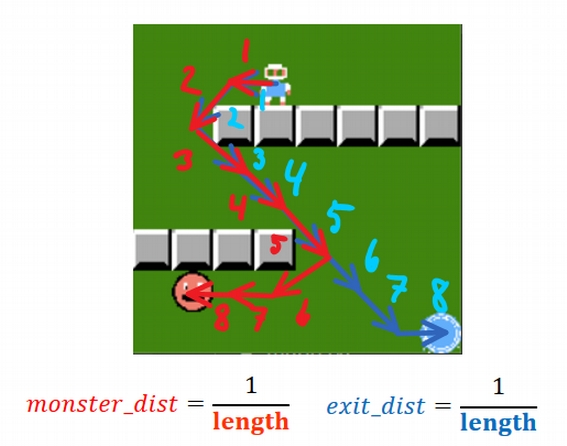
\includegraphics[height=4cm]{Writeup/dist_fn.jpg}
     \caption*{A* path distance function (monsters and exit)}
   \end{minipage}\hfill
   \begin{minipage}{0.48\textwidth}
     \centering
     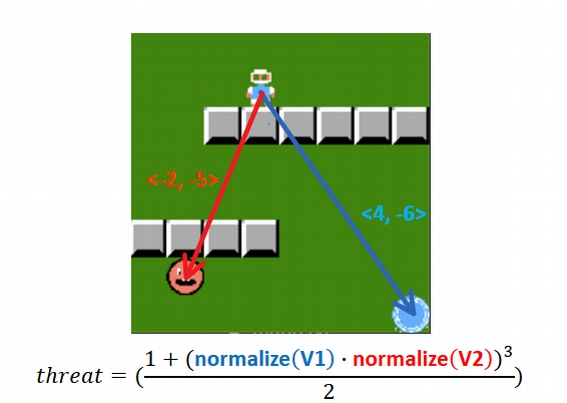
\includegraphics[height=4cm]{Writeup/threat_vec_fn.jpg}
     \caption*{Dot-product monster path threat function}
   \end{minipage}
\end{figure}


\begin{figure}[!htb]
   \begin{minipage}{0.48\textwidth}
     \centering
     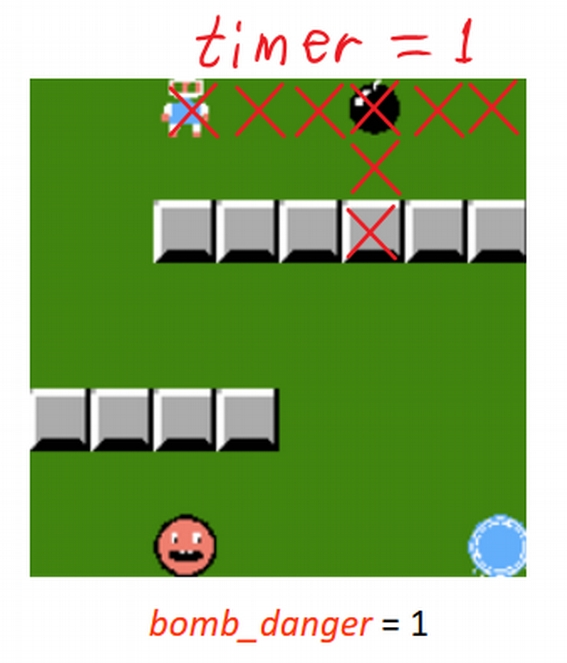
\includegraphics[height=4cm]{Writeup/bomb_danger_fn.jpg}
     \caption*{Bomb danger function}
   \end{minipage}\hfill
   \begin{minipage}{0.48\textwidth}
     \centering
     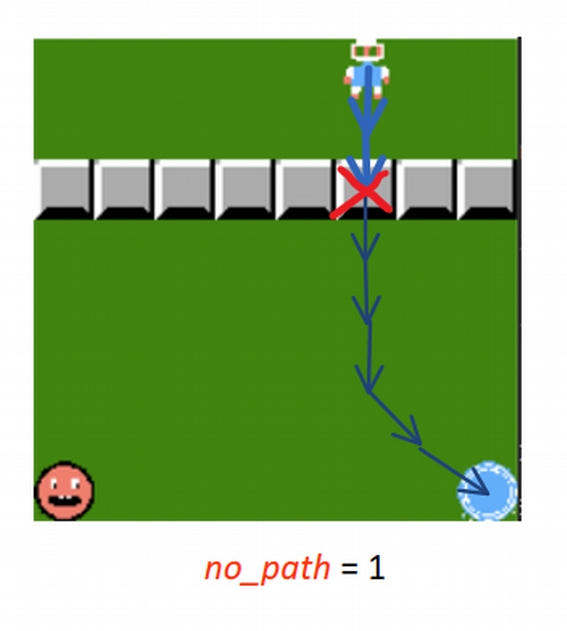
\includegraphics[height=4cm]{Writeup/no_path_fn.jpg}
     \caption*{Missing path function}
   \end{minipage}
\end{figure}


\subsection*{Training Structure}
To train our agent in dangerous situations, we constructed random training scenarios of 8x8 grids with different wall layouts as well as monsters randomly placed just within danger range. In each of these randomly generated scenarios, the agent would have to either move past the monster to the bottom of the grid, or kill the monster.
These situations were generated randomly, but after some initial testing, we selected certain map layouts which we found to be more difficult and representative of the real game for focused training.

\begin{figure}[h]
    \begin{minipage}{\textwidth}
      \centering
      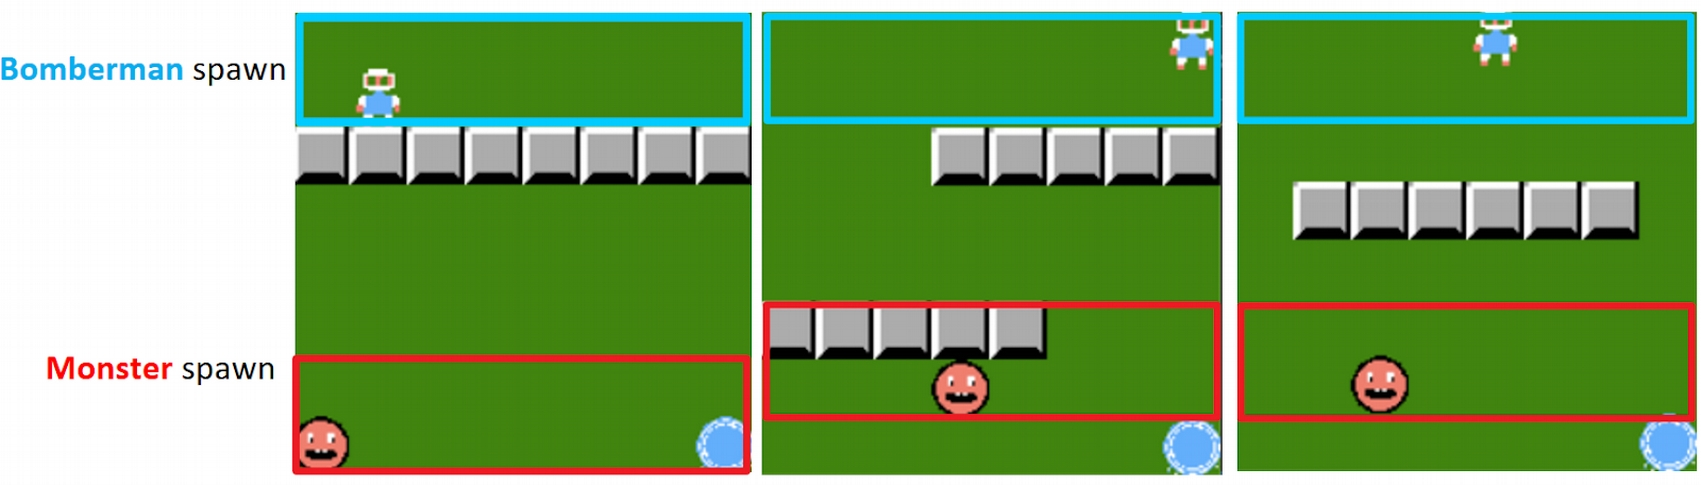
\includegraphics[width=0.85\linewidth]{Writeup/training_setup.jpg}
      \caption*{Random generation setup for training minigames}
    \end{minipage}
\end{figure}
\clearpage
\noindent Throughout our training, we used epsilon-greedy exploration, where we linearly decreased our epsilon from an initial value of 0.8 at varying speeds depending on how many generations we wished to train. We used a static learning rate (alpha=0.25), and we kept our rewards simple. We had large positive and negative rewards for passing the scenario and dying, respectively. We experimented with no cost of living, and with a small cost of living, and found that generally we would have more local maximums when we included a cost of living. We also included another reward for placing a bomb where it could break down a necessary wall.
We would run training sets for 250 and 500 generations, where each generation consisted of playing 9 of the randomly generated scenarios. We would then test the best-performing agents over these generations on the full set of scenarios, in combination with our safe A* agent.

\begin{figure}[h]
    \begin{minipage}{\textwidth}
      \centering
      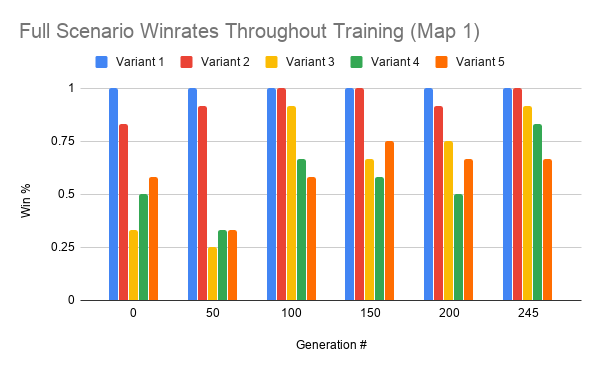
\includegraphics[width=0.65\linewidth]{Writeup/full_wr_training_map1.png}
      \caption*{Winrates throughout training on variants with the more open map}
    \end{minipage}
\end{figure}

\begin{figure}[h]
    \begin{minipage}{\textwidth}
      \centering
      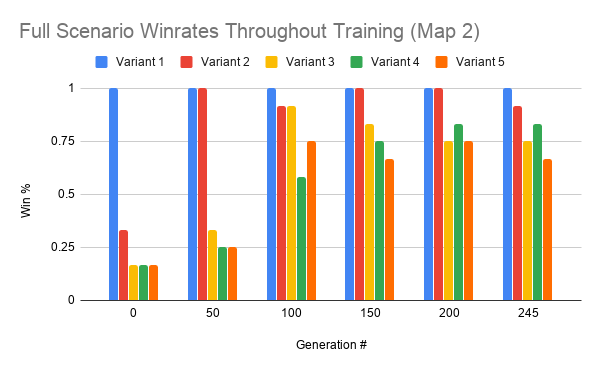
\includegraphics[width=0.65\linewidth]{Writeup/full_wr_training_map2.png}
      \caption*{Winrates throughout training on variants with the walled map}
    \end{minipage}
\end{figure}

\section{Results}
While the training produced an increasing win rate in the smaller training scenarios, things fared differently in the final scenarios. Depending on where monsters were located when our agent approached, it could find itself in unsolvable situations. For this reason, we tried modifying when the agent utilizes its intelligent behavior on a per-scenario basis. In the more problematic scenarios (open map, variants 4 and 5), we found some slight improvements by increasing the distance threshold for it to act as though it was in danger. These improvements were just enough to push us to the 80\% winrate threshold for the project, but in an ideal world we would have had the time to train a separate agent for these specific scenarios (focusing more on training in open maps with the most aggressive monsters).

\begin{figure}[h]
    \begin{minipage}{\textwidth}
      \centering
      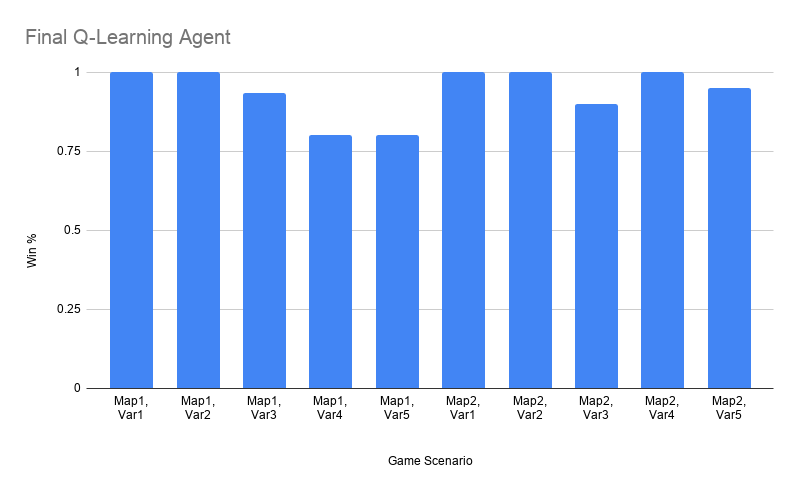
\includegraphics[width=0.95\linewidth]{Writeup/final_agent.png}
      \caption*{Winrates for final optimized agent}
    \end{minipage}
\end{figure}



\section{Reflection}
When confronted with a system housing many moving parts and even other AIs like we have in Bomberman, it is important to break the system down into discernible situations. While we initially sought to learn an all-purpose policy for the game, the resources available to us and the features we devised were not enough to learn such a solution. If we were to complete a similar project in the future, we would start by categorizing only what we need our agent to learn and develop training levels that specifically cater to those types of situations. This narrows the work into only a few smaller training sessions and a means for determining which distinct situation the agent is in.


\end{document}
